
\chapter{System Architecture, Design and utility frameworks}\label{chapter:SystemArchitecture}
In this chapter, we describe some highlights in terms of the architecture of the setup.  We start off by summarizing all the components we had described in Chapters \ref{chapter:DDPGFuncs}, \ref{chapter:ShockBuffer} and \ref{chapter:Estimates} with an architecture diagram and then a class diagram showing the compositional and hierarchical structure of the different classes we designed. We then proceed to give some comments about the architecture in broadly 4 areas
\begin{itemize}
    \item \textbf{Modular components of the setup}. The different components of the set up that can be 'plug and played' are.
    \begin{itemize}
        \item Actor 
        \item Critic 
        \item Replay Buffer
        \item DDPG Flavors
    \end{itemize}
    \item \textbf{Tracking , Visualization}. Combining good tracking tools such as MLFlow, we also have implemented a visualization framework based on dash \cite{dash_2022}, to see the list of results and export the data for charting, and a tailor made list of plot functions that can be extended to further projects that extend this idea.  
    \item \textbf{Deployment} - We present our Fastapi\cite{FastAPI} based server, from where experiments can be spawned directly from a webserver that can be hosted from any location.
    
    \item \textbf{Hyper parameter network}. We present a customizable tuning framework from where families of configurations can be launched from a configuration file.
    
\end{itemize}
\section{Architecture}
\begin{figure}[htpb]
\centering
  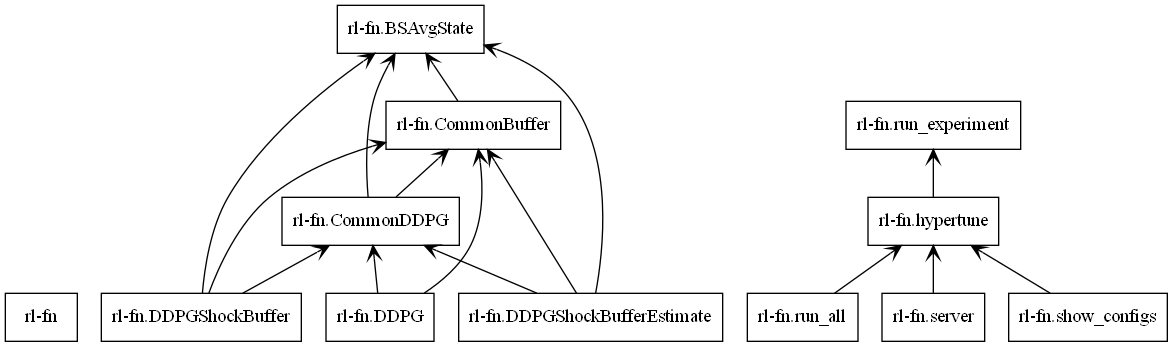
\includegraphics[width=1.0\textwidth]{figures/Results/rl-fn_architcture.png}
  \caption[Architecture]{Architecture of the different components in the project } \label{fig:architecture}
\end{figure}
There are 2 different kinds of components in the architecture specified in Figure \ref{fig:architecture} - the core DDPG components and the driver components.

The driver components broadly specify the different ways the project can be run. They are
\begin{itemize}
    \item \textbf{run\_all} : This is the traditional version of the project , a command line version from where the project can be run. The command line version takes a configuration file as input which contains the parameters of the experiments along with the hyper parameters, that have to be tuned and calls the \textbf{hypertune} component, which would spawn individual configurations for each value of a hyper parameter. The generated config would then be used by the \textbf{run\_experiment} module which would run individual experiments using the core components of the project.
    \item \textbf{server} : This is almost equivalent to the command line version in terms of the functionality but this is used while the project is hosted on a server, serving Restful APIs  \cite{fielding2000architectural} from a Flask framework \cite{UVicorn} 
    \item \textbf{show\_configs} : This version is used to only generate all the configurations, corresponding to all the tunable hyper parameters and would not run the individual experiments.  This version is ideal to inspect the possible configurations an experiment will be tuned for.
\end{itemize}
The core components encompass the different DDPG versions \textbf{DDPG}, \textbf{DDPG ShockBuffer}  and \textbf{DDPG Estimates} (shown as DDPGShockBufferEstimate in Figure \ref{fig:architecture}). The common functionalities for all these components are inherited in a \textit{base class}, \textbf{CommonDDPG}. All the 3 versions use the same replay buffer \textbf{CommonBuffer}, which is already customized to store the environment variables , extra variables such as log-returns (specific only to Shock buffer) and can be easily extended to store other parameters in any newer setting. The \textbf{BSAvgState} is the environment component that is used across all the other components and progresses the episodes of the experiments. The environment currently supports a Black-Scholes process and the utility functions - log and power. Besides the component can be extended to newer utility functions by overriding a utility interface in the environment class.   

The class diagram for these components is displayed in Figure \ref{fig:classdiag}.


\begin{figure}[htpb]
\centering
  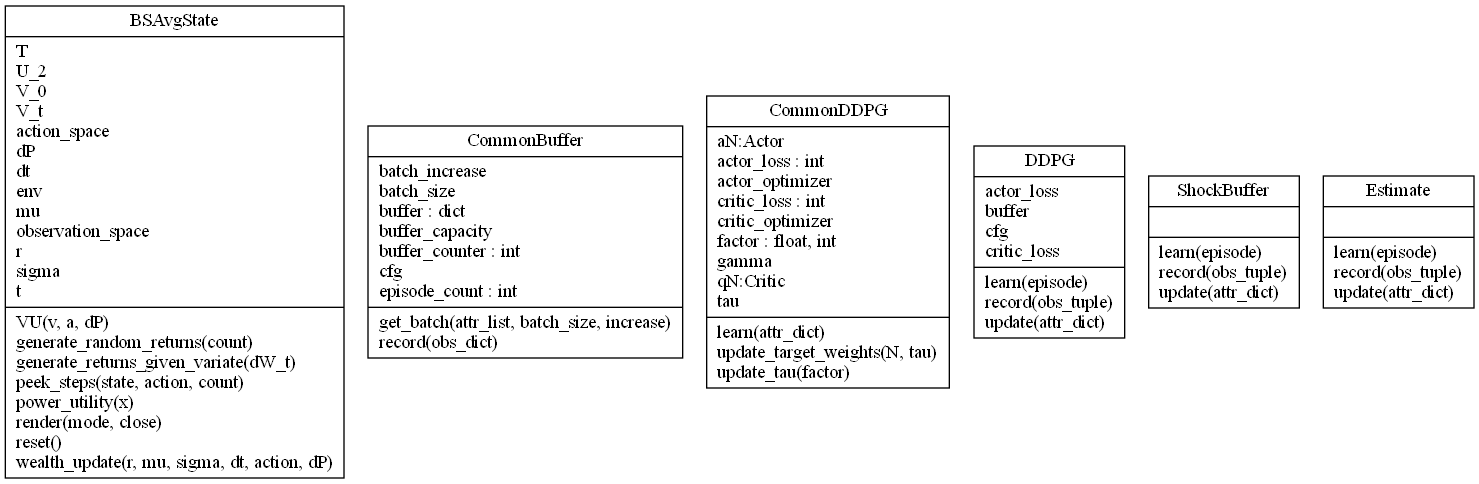
\includegraphics[width=1.0\textwidth]{figures/ClassDiagram.png}
  \caption[Class diagram]{Class diagram of DDPG components } \label{fig:classdiag}
\end{figure}
\pagebreak
Besides, we have a number of classes for the critic and the actor as well. There are 2 types of Q (and A) classes we use depending on how the critic and actor are defined. They are shown in Figure \ref{fig:classdiagc}.


\begin{figure}[htpb]
\centering
  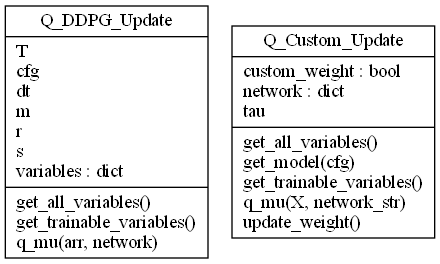
\includegraphics[width=1.0\textwidth]{figures/QClasses.png}
  \caption[Class diagram - Critic Functions]{Class diagram of critic } \label{fig:classdiagc}
\end{figure}
Q\_DDPG\_Update corresponds to cases (ii) and (iii) defined in Table \ref{table:actor_critic}, while Q\_Custom\_Update corresponds to case (i) defined in the same table.The difference between these 2 classes is that the Q\_Custom\_Update has an extra method update\_weight which needs to be customized for case (i).

\pagebreak
\section{Modular Components}\label{section:Modular Components}
At the heart of every experiment run is a configuration which we take as input.
A sample configuration is described below.
\begin{lstlisting}[language=json,firstnumber=1,caption=Example Configuration,label=json:sample_config]
{
  "name": "Experiment - Decaying tau and batch size in DDPG Shock Buffer version",
  "env": {
    "name": "BlackScholes-V2",
    "mu": 0.09,
    "sigma": 0.3,
    "r": 0,
    "T": 1,
    "dt": 0.2,
    "V_0": 1.0,
    "U_2": "pow",
    "b": -1
  },

  "general_settings": {
    "max_episodes": 5000,
    "max_steps": 100,
    "batch_size": 1024,
    "batch_size_increase": "linear"
  },
  "ddpg": {
    "type" :
       {
      "name": "DDPGShockBufferEstimate",
       "m": 20
       },
    "gamma": 1,
    "noise_decay": 1,
    "noise_scale": 1,
    "tau": 0.005,
    "tau_decay": "linear",
    "buffer_len": 20000,
    "q": {
      "name": "q_pow_utparametric",
      "lr": 0.005,
      "variables": [
        0.1,
        0.2,
        0.1,
        0.1
      ]
    },
    "a": {
      "name": "a_pow_ut1",
      "lr": 0.001,
      "variables": {
        "m": 0.1
      }
    }
  }

\end{lstlisting}

 As one can see in the Listing \ref{json:sample_config}, broadly there are 3 modules: 
 \begin{itemize}
     \item \textbf{Environment (env)}: This module takes the environment parameters, and a utility function as input. This includes $r,\mu$,$\sigma$, the time step interval $\Delta t$, T, initial wealth $v_0$ and the utility function $U$.
     
     The parameters are themselves quite flexible and new parameters can be added and existing parameters can be removed easily. For example one can set up a Heston model \cite{Heston1993}  instead of a Black Scholes Model by defining the evolution of the volatility explained by the equations
     \begin{equation}\label{HestonEq}
    \begin{array}{l@{}l}
     dS_t = (r + \eta z_t)S_tdt + \sqrt{z_t}S_tdW(t)\\
     dz_t = \kappa(\theta - z_t)dt + \sigma \sqrt{z_t}dW_z(t).     
     \end{array}
     \end{equation}
     In terms of our modular setup, we would have to redefine the step function as specified in the Algorithm \ref{alg:env_step} and then add the following variables :
     \begin{itemize}
         \item $\eta$ - Market price of the risk driver
         \item $\kappa$ - Mean reversion speed of volatility
         \item $\theta$ - Long-run average volatility
         \item $\sigma$ -  Volatility of volatility
         \item $\rho$ - Correlation factor
         
     \end{itemize} The other components of the DDPG can just 'flow' in as they were implemented.
     \item \textbf{DDPG}: 
     The DDPG module itself can be replaced by different flavors / implementation. What we described in Algorithm \ref{alg:ddpg_update} is only 1 version for our DDPG. As we have seen in Chapters \ref{chapter:ShockBuffer} and \ref{chapter:Estimates}, any DDPG model can be plugged in so long as it includes the following APIs
    \begin{itemize}
        \item Learn - The function that is meant to update the Q-value and a-value functions. 
        \item Record - The API that stores all the experience into a replay buffer.
    \end{itemize}
    Besides the APIs that DDPG should support, there are a bunch of hyper parameters that DDPG operates on, that are also listed in the sample configuration.
    \item \textbf{Actor($a$) and Critic ($Q$)}
        The different actor and critic algorithms that were discussed in detail in Chapter \ref{chapter:ExperimentSetup} are implemented in these modules. There is no restriction or a sense of constraint between the critic and the actor functions themselves. Any set of interesting modules can be used and experimented in the existing set up.
        We however require that these modules support the following APIs.
        \begin{itemize}
            \item The critic  should implement a function - Q\_mu(s,a) that returns the Q value of the state-action tuple, (s,a).
            \item The actor  should implement a function Mu(s) that returns the (suggested) optimal action for state 's'.
            \item The function TrainableVariables() for both actor and critic, that provides the list of variables to be trained using stochastic gradient descent in the context of DDPG.
            \item The function AllVariables() - A tuple of both trainable variables and the 'target' network variables that are not trained but just updated.
        \end{itemize}
 \end{itemize}
\section{Data Visualization, Experiment Tracking, Deployment and Plotting}
These are some of the downstream activities of our experiments but they are crucial to gain insights from the experiments we were conducting. Since the functions we chose for the actor and critic were quite small in terms of parameters compared to a multi-layered neural network, most of our experiments ran much faster compared to traditional DDPG problems.

Therefore we were able to run a vast number of experiments, tuning different hyper parameters, building  many versions of the core DDPG algorithm itself and also tracking the accuracy of our experiments in different environmental conditions - namely under different expected return and volatility of the risky assets.

Manually keeping track of so many experiments was hard and we were able to achieve better tracking by integrating MLFlow \cite{Zaharia2018MLflow} into our experiments. 

\subsection{Experiment Tracking and Visualization}

Here we present a dashboard that can be constructed from running many configurations in a particular experiment.

\begin{figure}[htpb]
\centering
  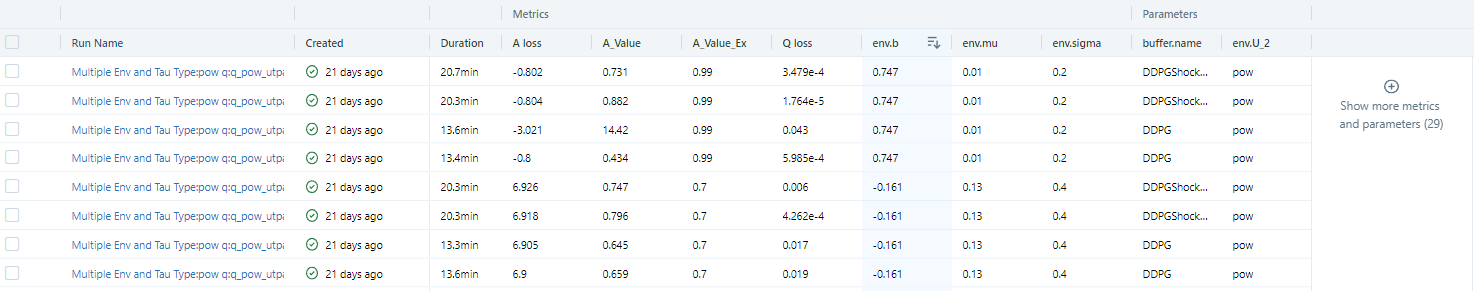
\includegraphics[width=1.0\textwidth]{figures/Dashboards.png}
  \caption[Sample Dashboard - Different Runs]{Sample dashboard showing the different runs of an experiment. Note A\_Value\_Ex is the theoretical optimal action } \label{fig:dashboard}
\end{figure}

The dashboard presents metrics, and parameters that can be logged during an experiment. Besides the metrics themselves, one can also log artifacts such as the configuration file mentioned in Listing \ref{json:sample_config}.

Within a run one can also see the progression of an experiment. The following plot shows the multi series of learned a-value, optimal a-Value, Q losses and a losses (i.e the maximization objective in the actor update) as we progress within an experiment.

\begin{figure}[htpb]
\centering
  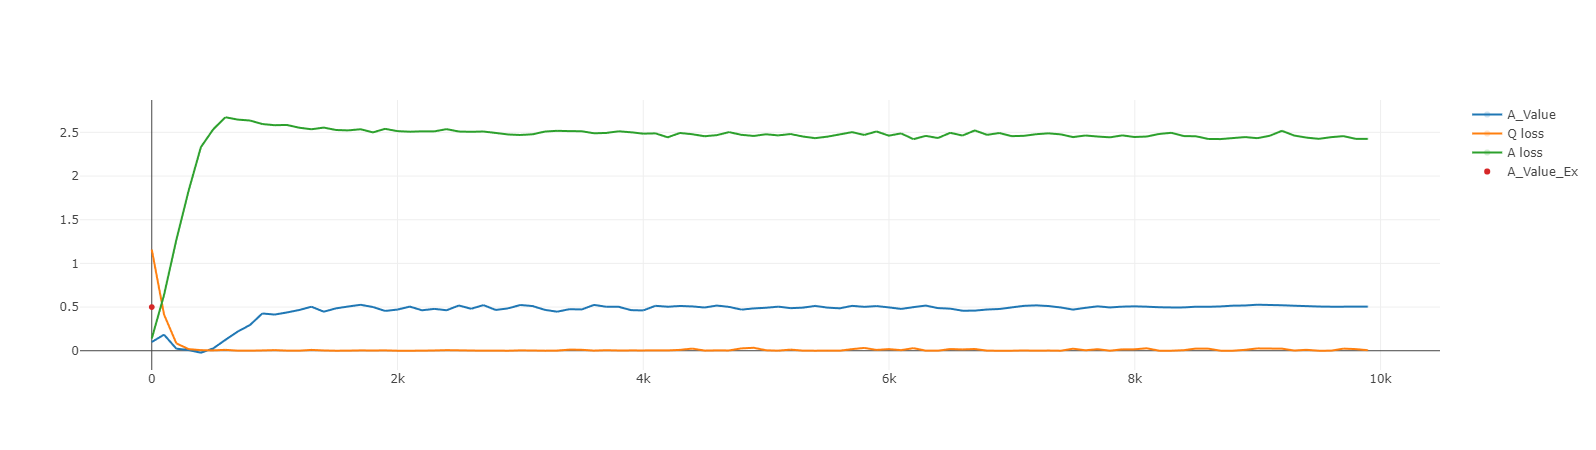
\includegraphics[width=1\textwidth,height=8cm]{figures/Losses.png}
  \caption[Sample Dashboard MLFlow]{Sample plots generated by MLFlow. } \label{fig:dashboard}
\end{figure}

Further, we also generated a customizable framework to create even more filters for our dashboards that MLFlow did not support. Our customizable framework is based on dash \cite{dash_2022} and a sample screen shot of that is found in Figure \ref{fig:DashDashboard}. We also hosted this framework at https://ddpg-po-dash1.herokuapp.com/ so that it is accessible everywhere. The difference between the framework is that the dash framework (implemented from scratch in terms of layout), has better filtering capabilities, and is much faster compared to the MLFlow UI. The layout has been improved to consider the specifics of the problem statement.
The following features are supported in the implemented dash framework in addition to the ones supported by MLFlow

\begin{itemize}
    \item Selecting multiple experiments to conduct experiments
    \item Visualizing summary statistics on the filtered experiments
    \item Visualizing losses in any particular experiment.
    \item Exporting the datatable to a comma separated value file.
\end{itemize}
Some screenshots of the application are shown in Figures \ref{fig:DashDashboard} and \ref{fig:dashboard-dash}

 \begin{figure}[!tbp]
  \subfloat[Filter ][Filter experiments]{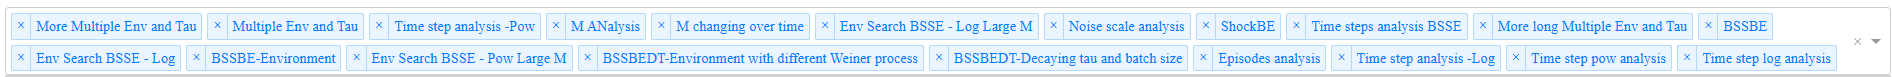
\includegraphics[width=1\textwidth]{figures/Filter.png}}
  \vfill
  \subfloat[Summary statistics ][Summary statistics]{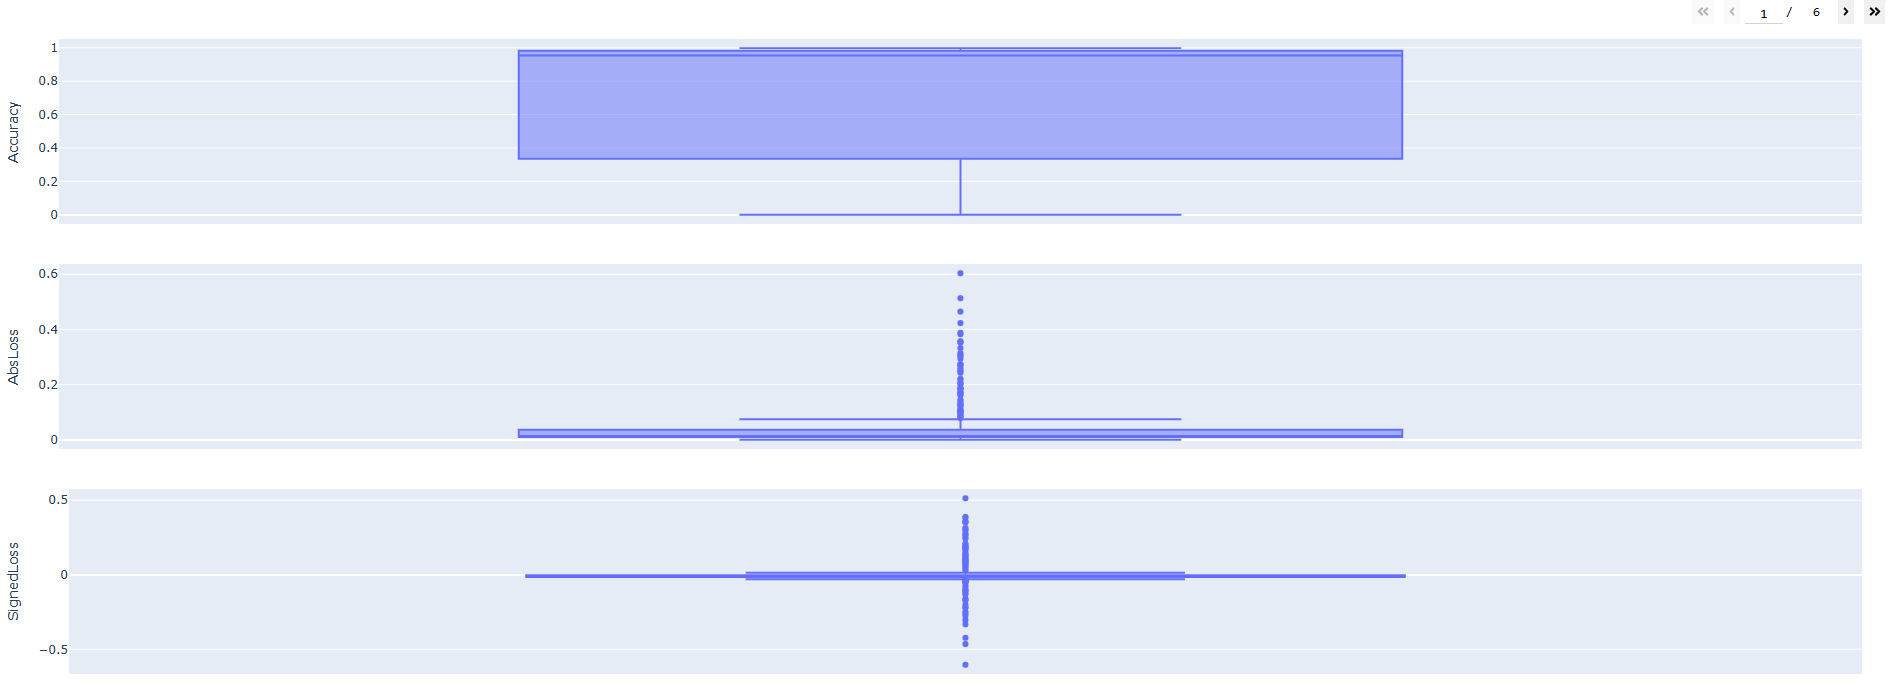
\includegraphics[width=1\textwidth,height=0.2\textheight]{figures/SS.png}}
  \vfill
  \subfloat[Losses ][Loss plots]{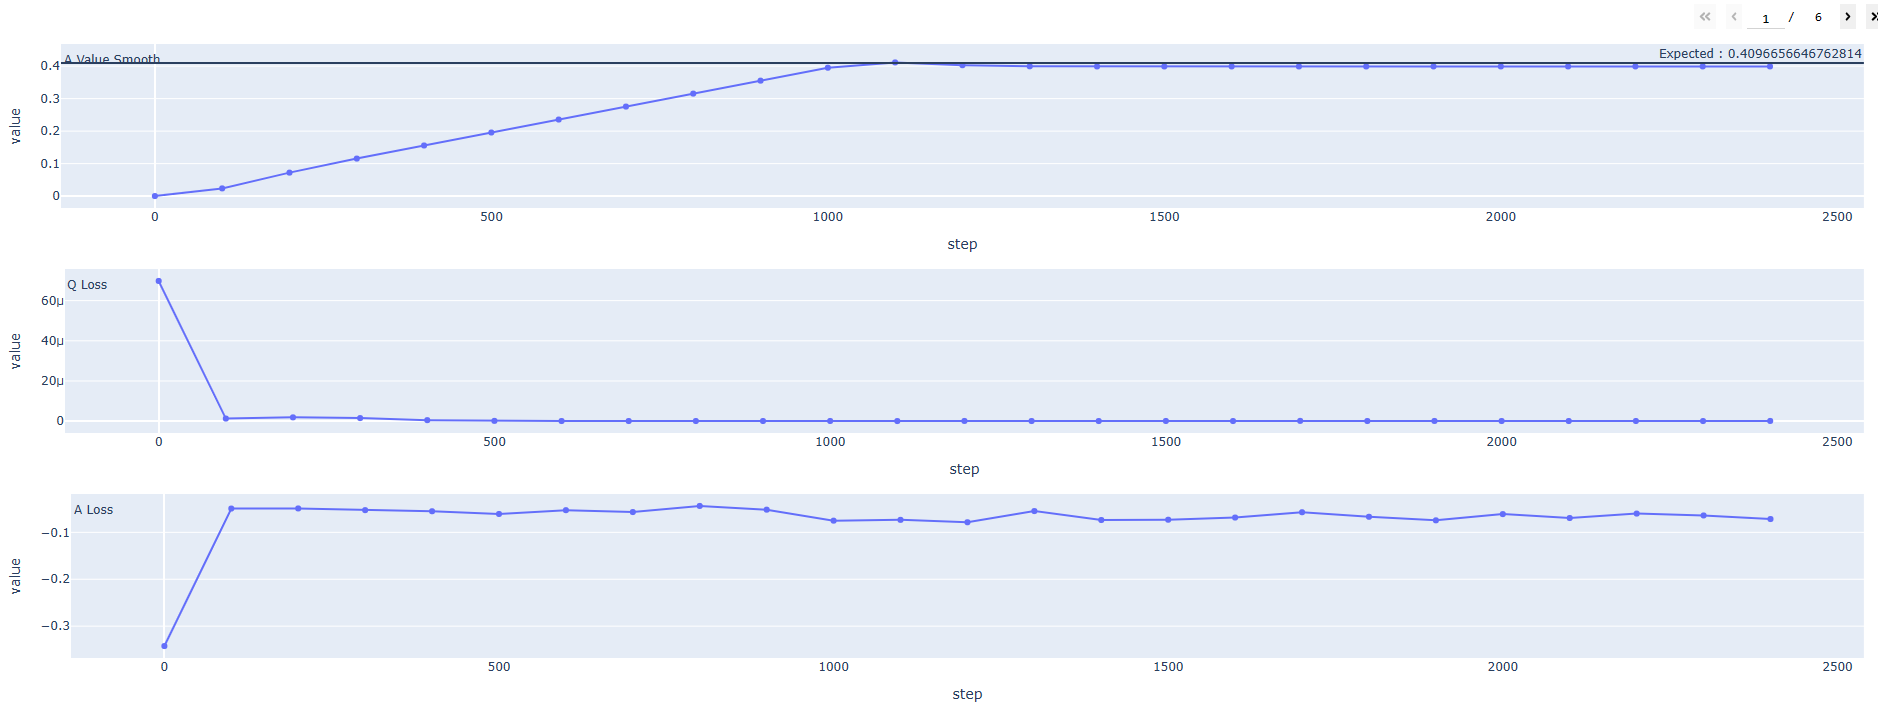
\includegraphics[width=1\textwidth,height=0.2\textheight]{figures/Plots.png}}
  \caption{ Dashboard screenshots}
  \label{fig:DashDashboard}
\end{figure}


\begin{figure}[htpb]
\centering
  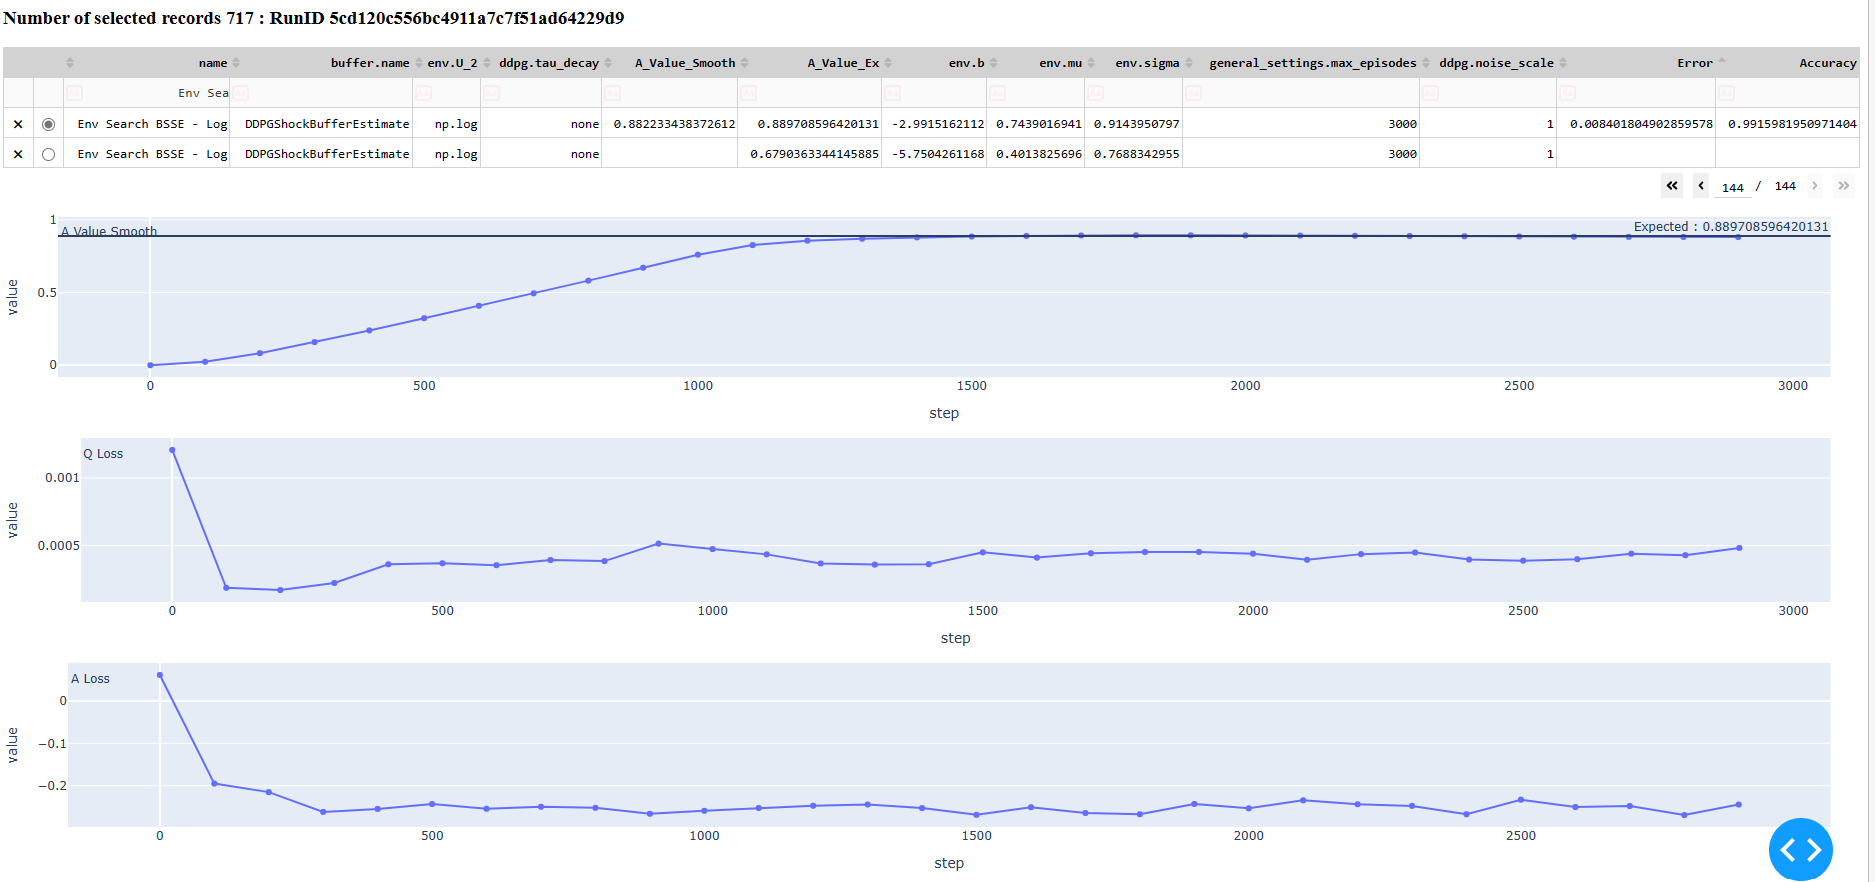
\includegraphics[width=1\textwidth,height=12cm]{figures/DashBoord-Dash.png}
  \caption[Sample plots -MLFlow Dash]{Sample plots generated by MLFlow - Dashframework} \label{fig:dashboard-dash}
\end{figure}

\pagebreak
\subsection{Deployment}
    To deploy the experiments, we implemented a framework based on the fastapi \cite{FastAPI} package. A Fastapi server is spawned using uvicorn - which is an ASGI web server implementation for Python \cite{UVicorn}. One can deploy a simple experiment or even a configuration of networks using the framework described in the next section \ref{section:hyp_parameter tuning framework}. 

    We show an experiment spawned and the resulting feedback in Figures \ref{fig:depl1} and \ref{fig:depl2}.
    
\begin{figure}[htpb]
    \centering
    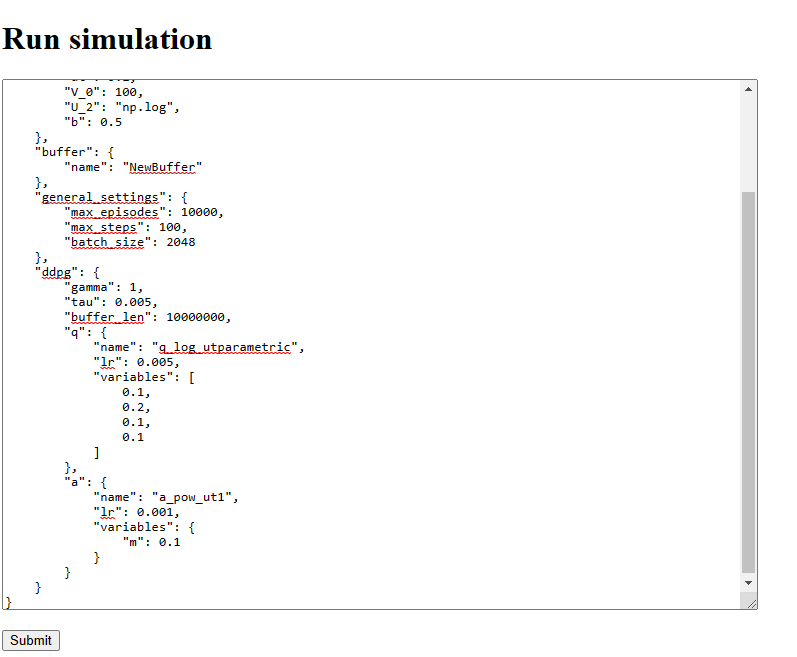
\includegraphics[width=0.5\textwidth,height=7cm]{figures/fastapi_deployment.png}
  \caption[Deployment step]{Deployment step } \label{fig:depl1}
\end{figure}
\begin{figure}[htpb]
    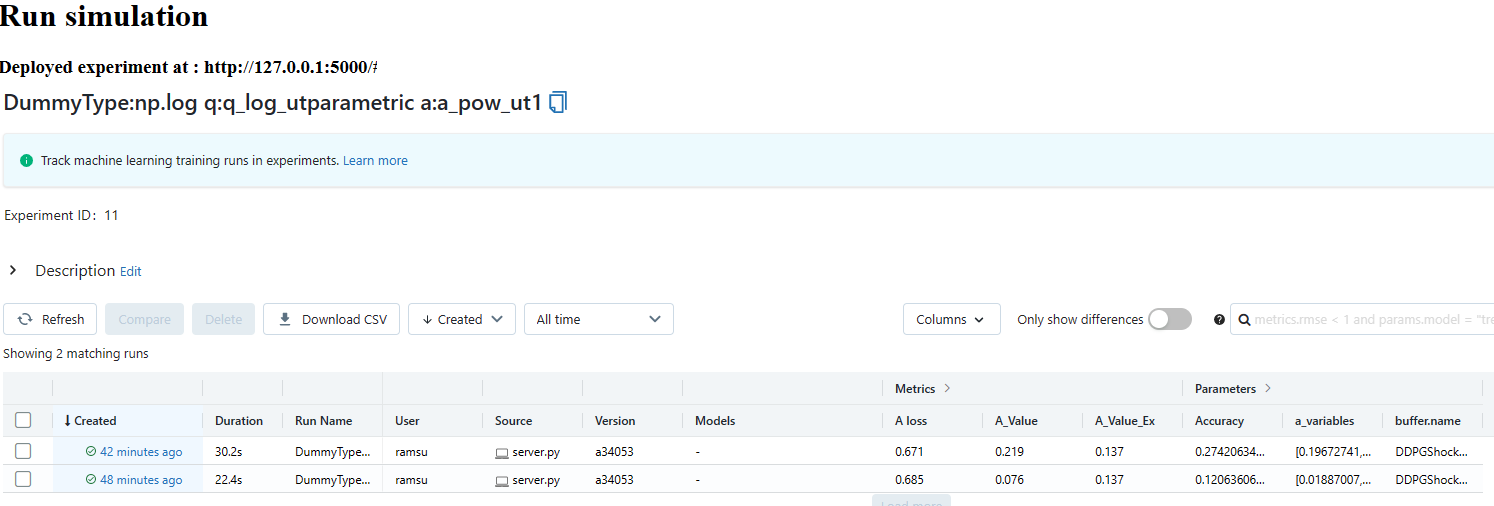
\includegraphics[width=1\textwidth,height=6cm]{figures/DeploymentResult.png}
  \caption[Deployment pipeline]{Deployment pipeline } \label{fig:depl2}
\end{figure}

\pagebreak

\section{Hyperparameter Tuning Framework} \label{section:hyp_parameter tuning framework}
One of the key requirements of the project is to conduct experiments across a large set of parameters. Some of the parameters could be environmental settings, such as the model parameters of the environment, the number of time steps to conduct an experiment, and the utility functions we need to try.

In addition, the hyper parameters of the algorithm itself could be a number of settings. For example  the parametric functions for the critic and actor, the learning rates used for the optimizing critic and actor loss, the target network learning rate $\tau$ among many others can all be changed leading to an exponential number of configurations. 

However in this section, we talk about a framework we implemented -  a configuration based approach to iterate through the different configurations of the optimization. Every base configuration specified in Listing \ref{json:sample_config} can be tuned with a tuning dictionary. A sample tuning is provided in Listing \ref{json:sample_tune_config_2}. \pagebreak
\begin{lstlisting}[language=json,firstnumber=1,caption=Tuning dictionary,label=json:sample_tune_config_2]
    "tune": {
      "buffer.name": {
        "list": [ "DDPGShockBuffer","DDPG"  ]
      },
      "env.dt" :
      {
        "list" : [ 0.01,0.02,0.1,0.2]        
      },
      "ddpg.max_episodes" :
      {
         "low" : 2000, "high" : 20000 , "step" : 100
      },
      "env.V_0"
      {
        "set" : "np.random.rand()*2" ,"size" : 10
      },
      "group":[
        {
          "env.mu": 0.019536,"env.sigma": 0.377183
        },
        {
          "env.b": -8.381621,"env.sigma": 0.57196
        }
      ],
      "group_2" :
      [
        {
        "ddpg.q.name" : "q_log_utparametric", "env.U_2" : "np.log"
        },
        {
          "ddpg.q.name" : "q_pow_utparametric","env.U_2" : "pow"
        } ]}

\end{lstlisting}
 In general every parameter specified in the configuration can be tuned. For example in the dictionary specified in 
 Listing \ref{json:sample_tune_config_2}, one of the ways the experiment can be iterated is over the time step, env.dt [See line 7]. Some of the ways the parameter can be tuned are specified below.

 \begin{itemize}
     \item \textbf{list} - By specifying list, we iterate over a set of specified values. Continuing on the example \ref{json:sample_tune_config_2} env.dt is iterated over the list { 0.01,0.02,0.1,0.2 }.
    \item \textbf{range} - By specifying the keyword,"low", and the optional parameters, "high" (default 1) and "step" (default 1) we specify a range [low,high,step] where we do a grid search for the hyper parameter from low to high incremented at each iteration by step.
    \item \textbf{set} - Set helps to evaluate an expression for the hyper parameter. The expression is any valid python based expression that returns a value compliant to the variable that it is being assigned to. In the Listing \ref{json:sample_tune_config_2}, we set $env.V_0$ the initial wealth by calling the expression "np.random.rand()*2" , 10 times.
    \item \textbf{group*} - While tuning hyper parameters, one can specify the level of granularity to iterate over by introducing "group" elements. If we do not have this element and tune over $n$ hyper parameters, then the total number of configurations generated would be $\prod_{i=1}^n C_i$ where $C_i$ is the number of values to be tested for a hyper parameter i. However, it makes sense to bunch a set of hyper parameter configurations together and iterate over another set of hyper parameters, along with them.
    
    For example, consider that we have 2 utility functions to be tested - power and log. And let the corresponding Q-value functions to be experimented are $Q^{\theta^p_i}$ and $Q^{\theta^l_j}$ respectively (where $1 \leq i \leq N_p$ and $1 \leq j \leq N_l$ ; $N_p$ and $N_l$ are positive integers). It would make sense to create a group with the power utility function and the different Q-value functions $Q^{\theta^p_i}$, and then create another group with the log utility function and  the different Q-value functions $Q^{\theta^l_j}$, instead of iterating over all possible configurations. This is possible with the "group" construct. Group elements should start with the prefix "group".
    The number of possible configurations would be $\prod_{i=1}^n G_i$ where $G_i$ is the number of configurations for a group $G_i$.  Note that  $\prod_{i=1}^n G_i \leq \prod_{j=1}^N C_j$. An element stated explicitly (as in the  examples for list, set and range)  is a group of one element trivially.
    Again within a group, one could recursively tune for list, set and range as discussed before and even have nested group variables inside it.
\end{itemize}



 